\section{Model Description \label{sec:model}}

\begin{figure}[htbp]
   \centering
   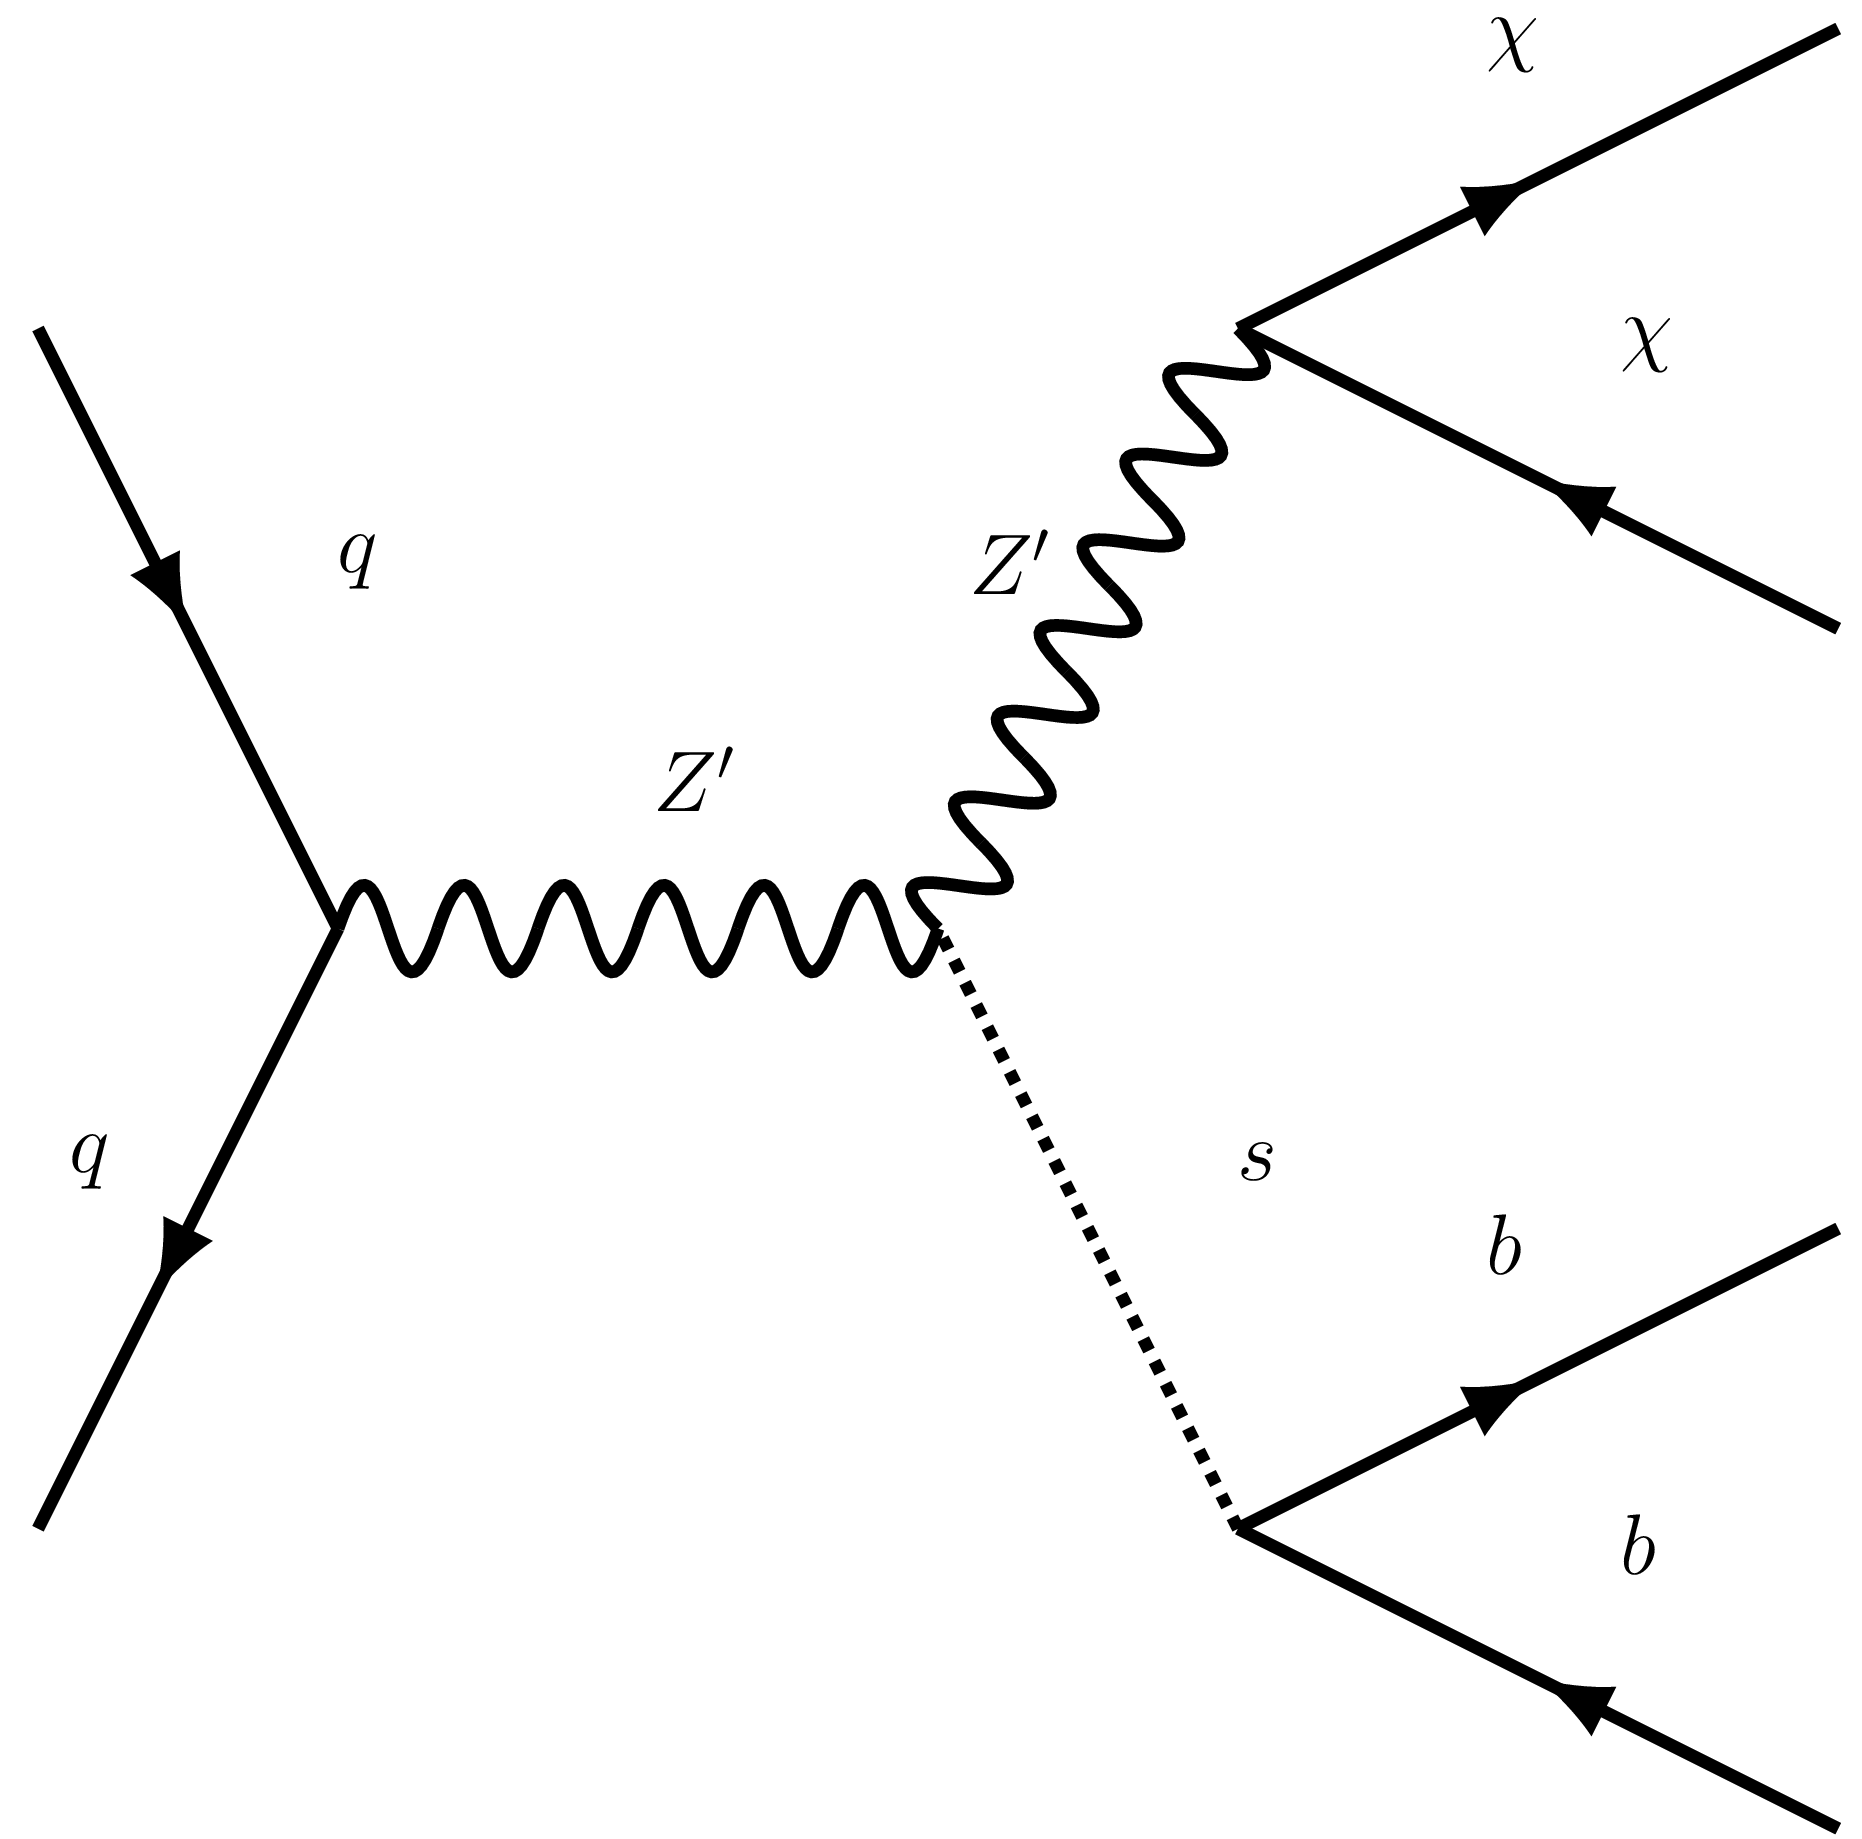
\includegraphics[width=0.5\textwidth]{figures/feyns/mono-hs.pdf}
   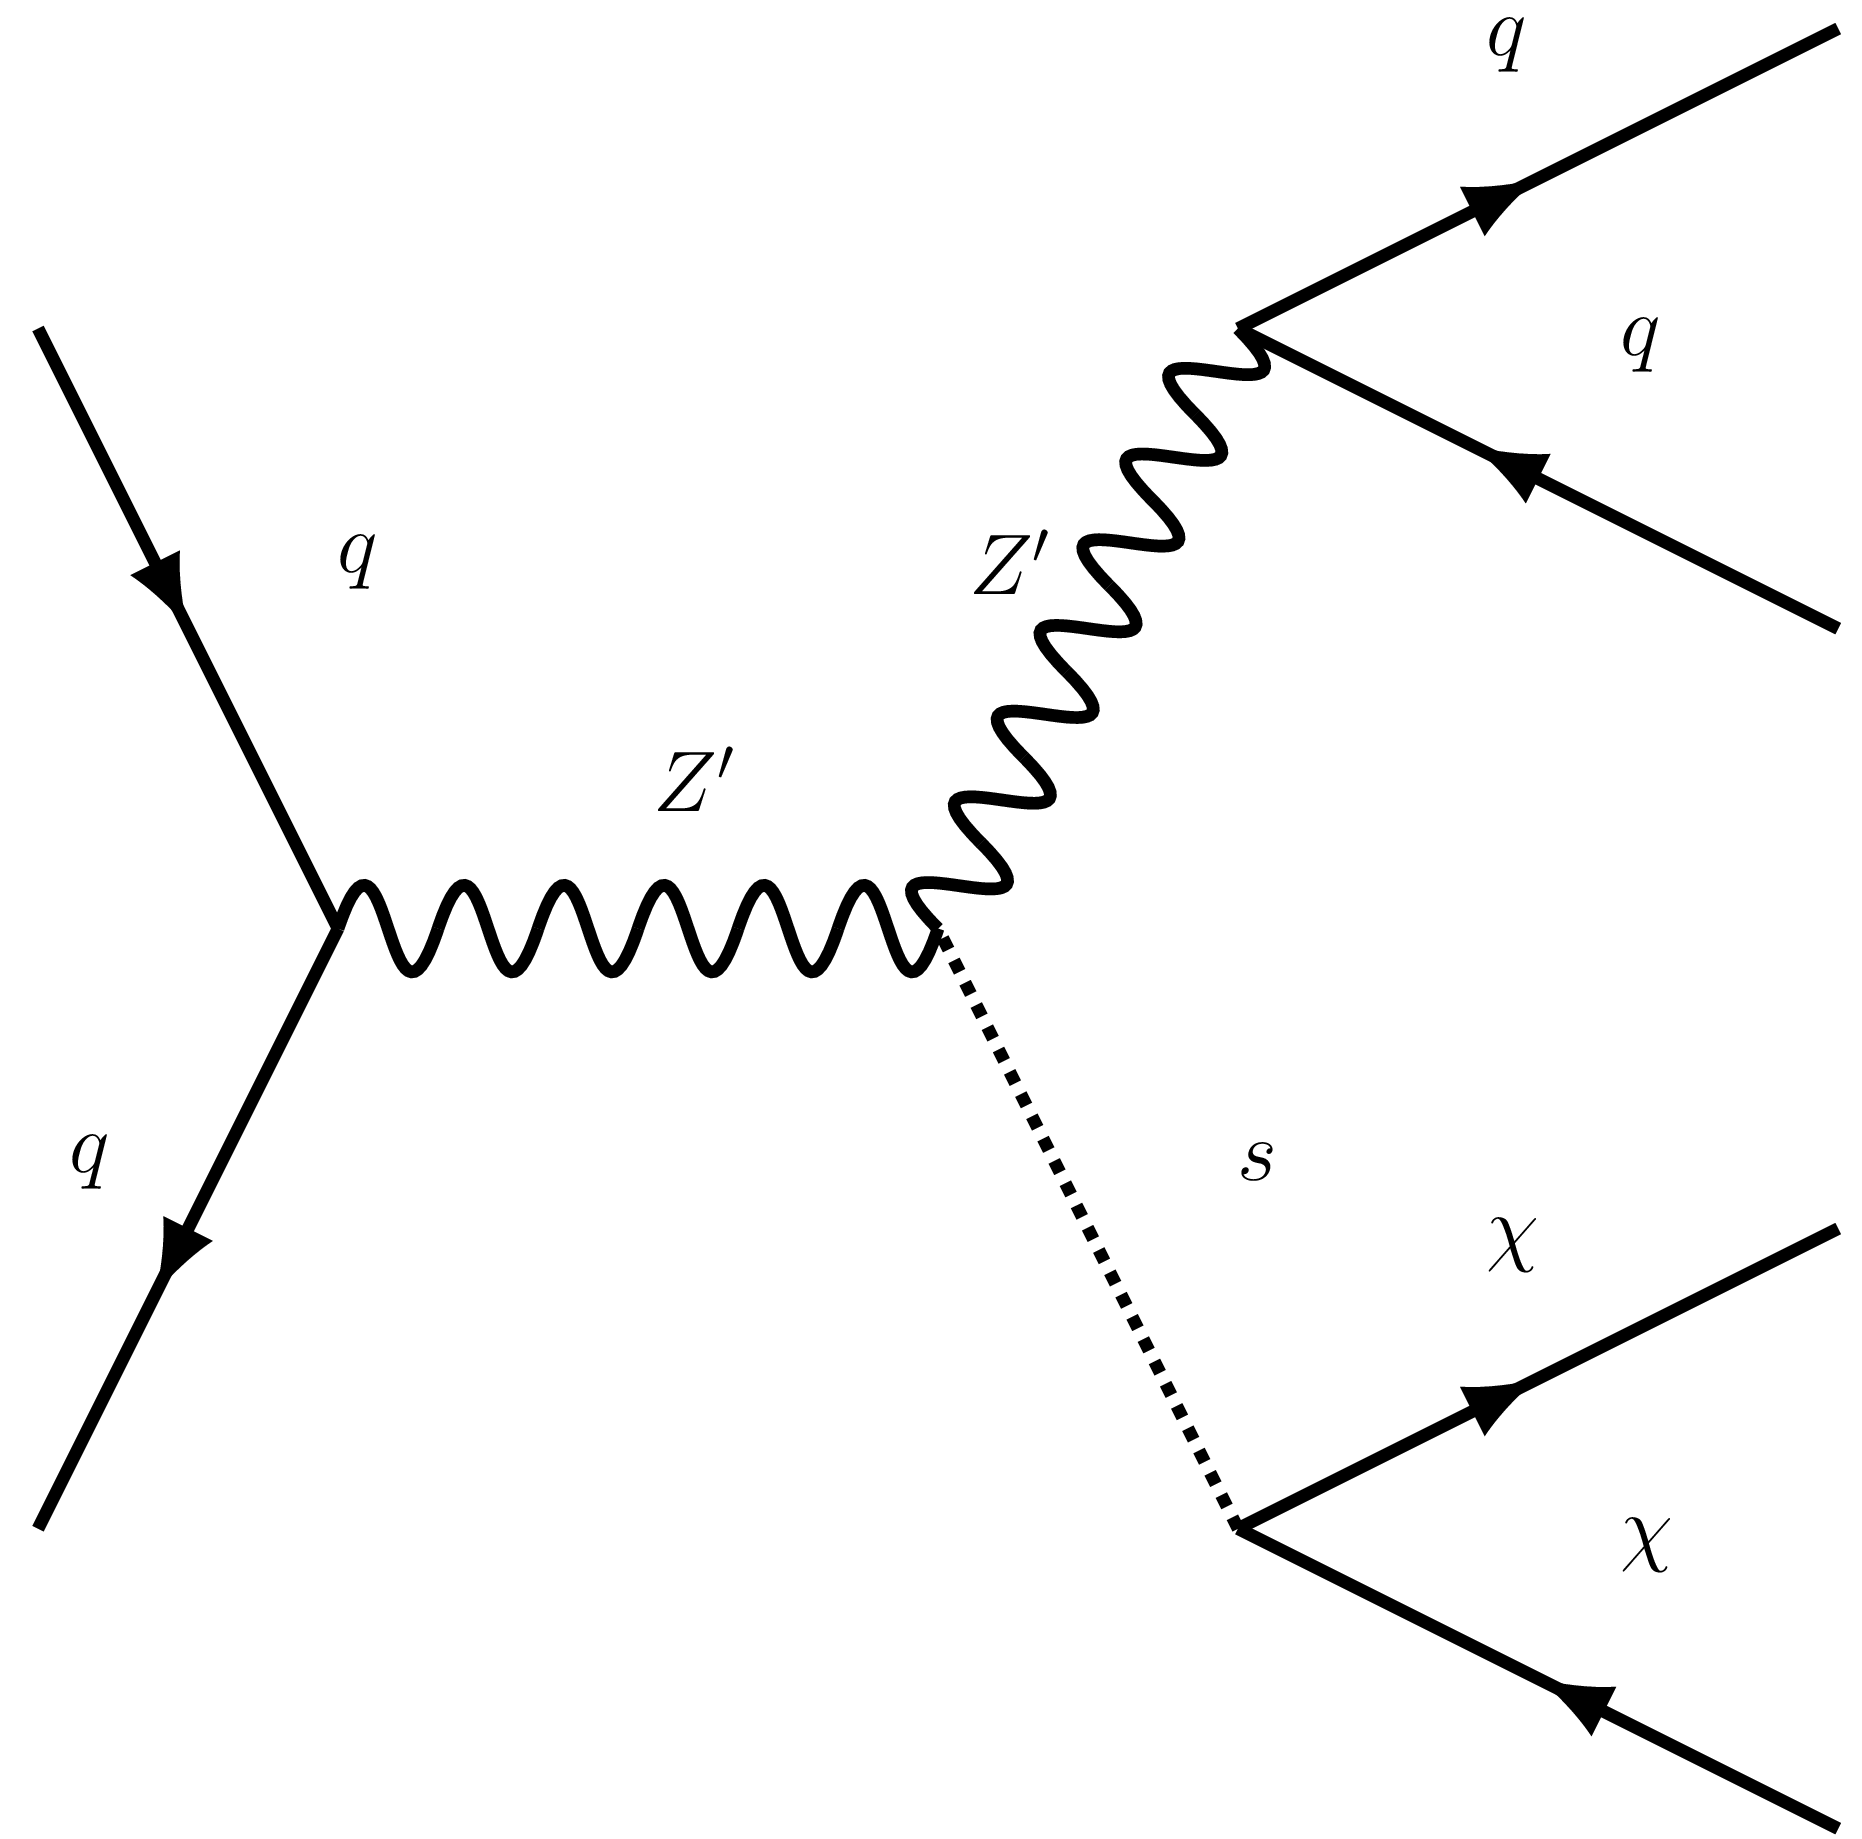
\includegraphics[width=0.5\textwidth]{figures/feyns/mono-Zp.pdf}
   \caption{Left: Feynman diagram of a visible dark Higgs production final state. Right: Feynman diagram of a visible Z' final state. Both proceeded with an off-shell Z' mediator with dark Higgs boson radiated off and eventually decay into SM final state. Both final states give rise to highly boosted jet with \MET signature.}
   \label{fig:feynman}
\end{figure}

We consider a Majorana DM particle $\chi$ that obtains its mass from the vacuum expectation value (vev) $w$ of a new complex Higgs field $S$, which is a singlet under the DM gauge group. The field $S$ carries a charge $q_{S}$ under a new $U(1)^{\prime}$ gauge group, so its vev $w$ breaks the gauge symmetry spontaneously and generates the mass of the corresponding $Z^{\prime}$ gauge boson. The symmetry breaking gives rise to a new physical Higgs boson. Under the dark Higgs model~\cite{Duerr2017}, the DM particle acquires an axial coupling to the $Z^{\prime}$, so that all three particles in the dark sector couple to each other.

We will be interested in the case where the DM particle is not the lightest state in the
dark sector, so that it can annihilate into other dark sector states which subsequently decay
into SM states. Scenarios in which the $Z^{\prime}$ is the lightest particle are typically disfavoured,
because they require the couplings of the dark Higgs boson to be close to the perturbativity
bound~\cite{Bai2015,PhysRevD.92.035007}. We therefore focus on the more natural case that the dark Higgs boson is the
lightest state in the dark sector and the relic density is largely set by the process $\chi\chi\rightarrow ss$.

The two mediators offer three different possibilities in which such a dark sector can
be coupled to the SM: via direct couplings of the $Z^{\prime}$
to SM particles, via mixing of the $Z^{\prime}$ with the neutral gauge bosons of the SM or via mixing between the dark Higgs boson and
the SM Higgs boson. In particular, non-zero mixing between the dark Higgs boson
and the SM Higgs boson ensures that the dark Higgs boson is unstable even if it is the
lightest state in the dark sector and decays into SM states with a negligible lifetime. The
required mixing angle can however be so small that it does not lead to any other observable
effects. For the purpose of this work we assume that the dominant interaction results from
vector couplings  of the $Z^{\prime}$ to quarks, which naturally arise in models of gauged baryon
number. 

There is also an obvious similarity to the spin-1 simplified DM model studied by the
LHC collaborations~\cite{Kahlhoefer2016}, with the one addition that we specify the mechanism
responsible for generating the masses of the DM particle and the $Z^{\prime}$ and for this purpose
introduce a dark Higgs. Since the couplings of the dark Higgs boson are fully specified
by the other parameters in the model, the only new parameter is the dark Higgs mass $m_{s}$. In order to be consistent with the benchmark introduced from ATLAS-CMS DM forum~\cite{Abercrombie:2015wmb}, we adopt $g_{q}$ = 0.25 and $g_{\chi}$ = 1.

With the requirement on the choice of coupling which allows to make contact with existing DM searches at the LHC, the observed DM relic abundance is only reproduced for certain combinations of the masses of the particles in the dark sector.

%\subsection{ \cPZpr-Baryonic model}
%A Z' vector boson is a well-motivated feature of many new physics scenarios. 
%The Z'-motivated DM models are more interesting since the corresponding U(1)' 
%gauge symmetry ensures DM stability. The model is an extension of the SM and 
%assumes that the baryon number (B) is gauged, with the Z' being the gauge 
%boson of U(1)$_{B}$. The consistency of theory requires the existence of new 
%stable baryonic state that are neutral under SM gauge symmetry. This new 
%particle is an excellent DM candidate. If the DM particle carries a baryon 
%number $B_{\chi}$, the Z'-quark-DM part of the Lagrangian for models with 
%fermionic dark matter is 
%\begin{equation}
%{\cal L} = g_q \bar{q}\gamma^{\mu}q\cPZpr_{\mu}+g_{\chi}\bar{\chi}\gamma^{\mu}\chi\cPZpr_{\mu}
%\end{equation}
%To generate the Z' mass, a ``baryonic Higgs'' scalar is introduced to 
%spontaneously break the U(1)$_B$ symmetry. Analogous to the SM, there remains 
%a physical baryonic Higgs particle, $h_{B}$, with a coupling of h$_{B}$Z'Z' 
%and vacuum expectation value of v$_{B}$. 
%The \cPZpr\ and SM Higgs boson h interact with a coupling strength of 
%$g_{h\cPZpr\cPZpr} = m_{\cPZpr}^{2} \sin \theta/v_{B}$, where $\theta$ is the h-h$_{B}$ 
%mixing angle. This allows for mono-Higgs final states at the LHC as shown in 
%Fig.~\ref{fig:feynman}. In the search for this model, values for $g_q$ and $g_\chi$ are chosen to be 0.25 and 1, respectively. The ratio $g_{h\cPZpr\cPZpr}/M_{\mathrm{Z}'}$ is chosen to be unity. All these parameter choices follow the recommendations from~\cite{Abercrombie:2015wmb}.  



%\begin{figure}[htbp]
%   \centering
%   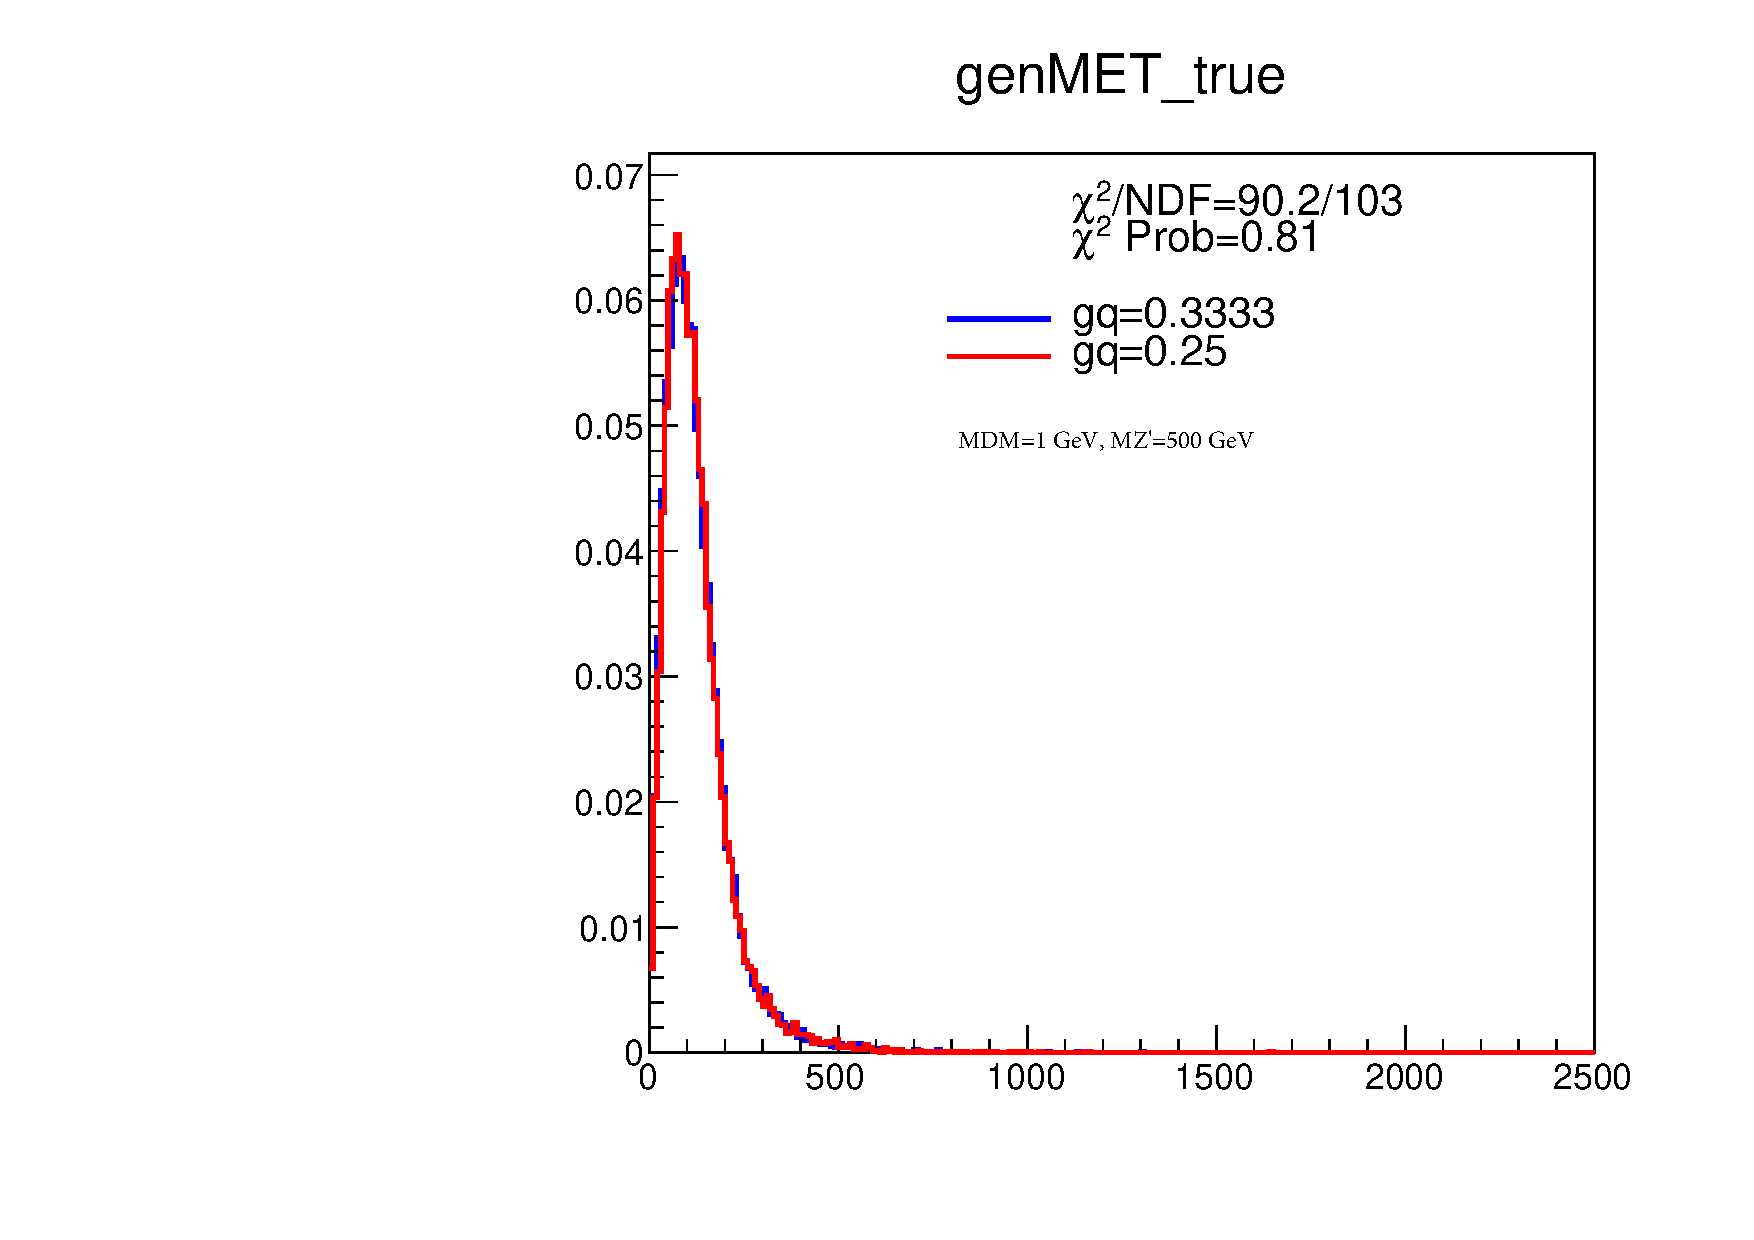
\includegraphics[width=0.7\textwidth]{figures/models/gq0p3333_ZpBaryonic_MSC500_MDM1_gq0p25_ZpBaryonic_MSC500_MDM1.pdf}
%   \caption{Comparison of the generator-level \MET\ distributions predicted 
%by the \cPZpr-Baryonic model (after parton shower by \PYTHIA) for $g_q=0.25$ and $g_q=0.3333$. The mass of 
%the dark matter particle is set to 1~\GeV and the mass of the mediator 
%\cPZpr\ is set to 500~\GeV, respectively. Samples for this model have been generated with $g_q=0.3333$; however, as the kinematics does not change, we% use them to interpret the results under the assumption $g_q=0.25$ by appropriately rescaling the cross section.}
%   \label{fig:METZpBgq}
%\end{figure}

%\begin{figure}[htbp]
%   \centering
%   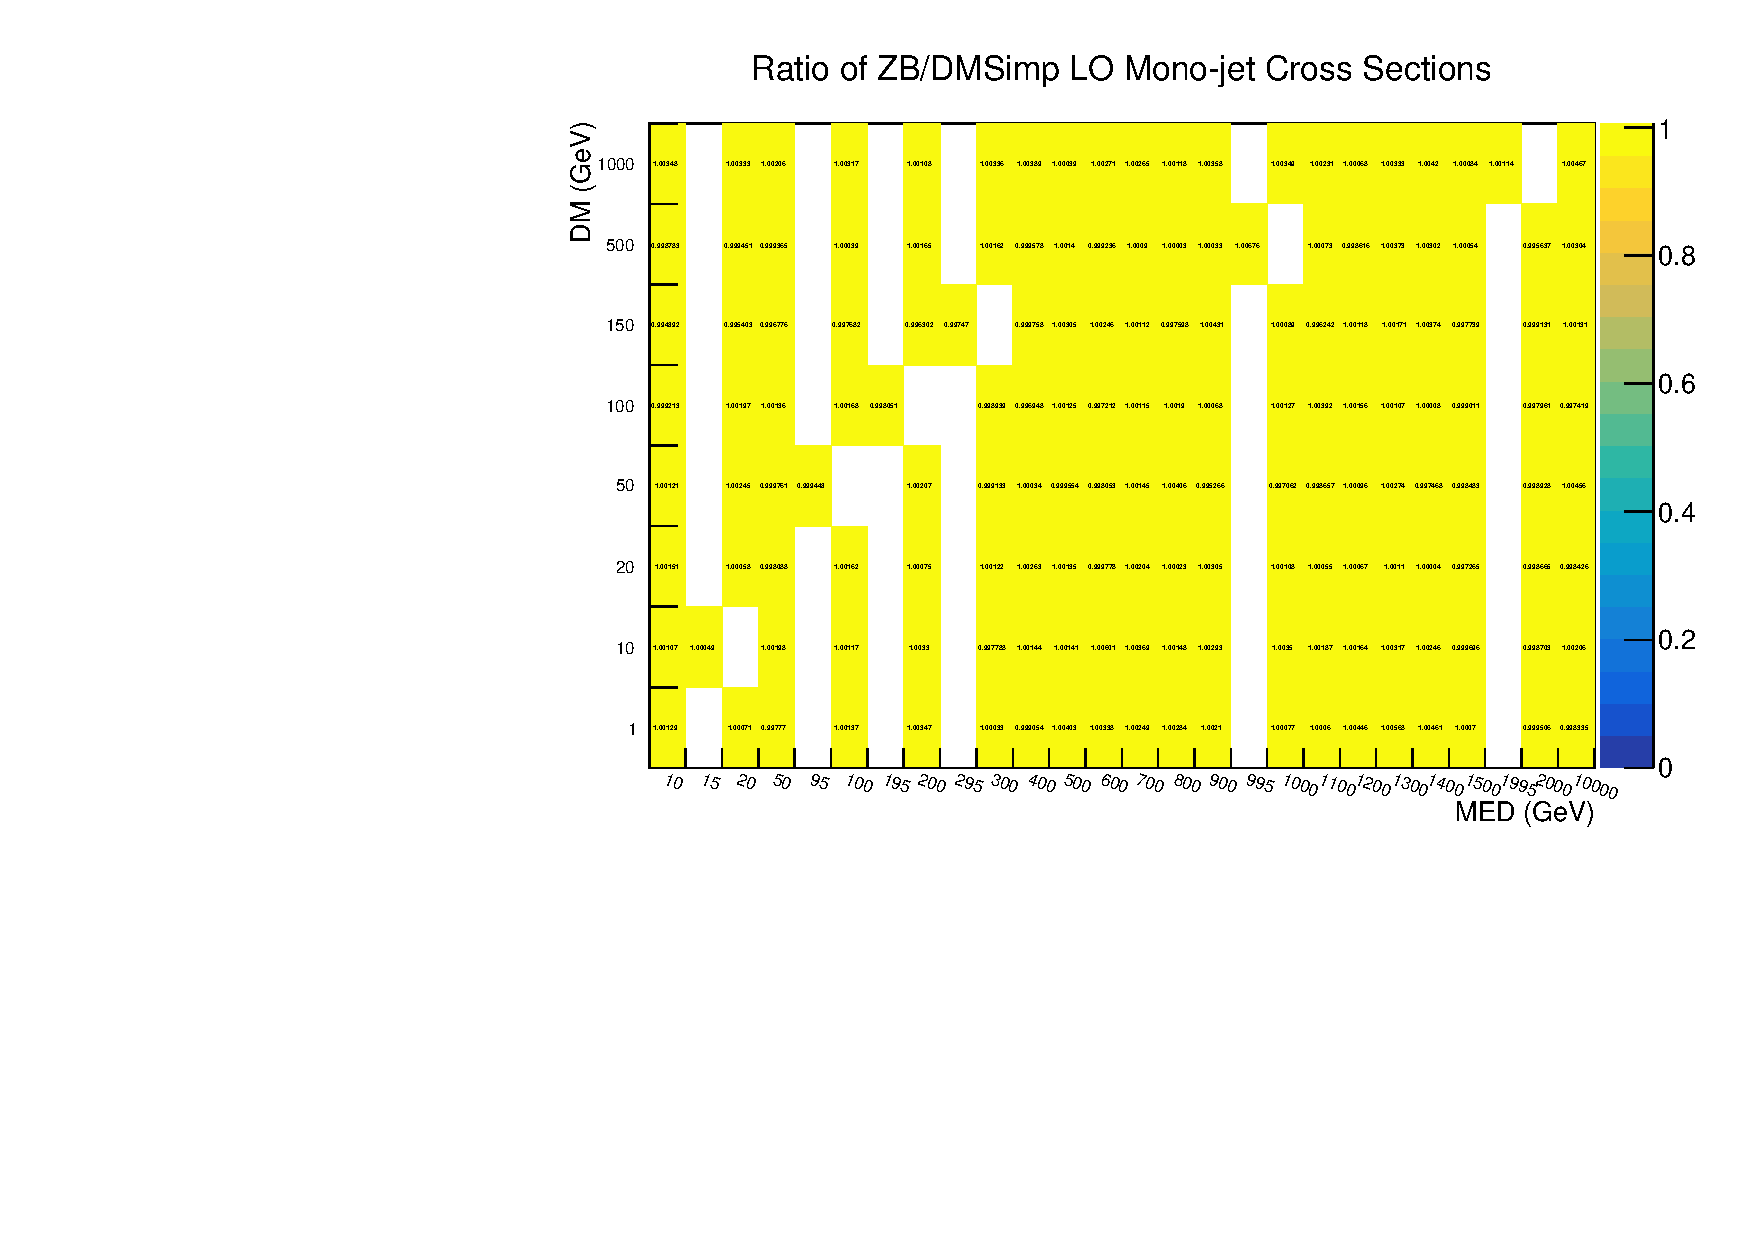
\includegraphics[width=0.45\textwidth]{figures/models/xsec_ZBToDMSimp.pdf}
%   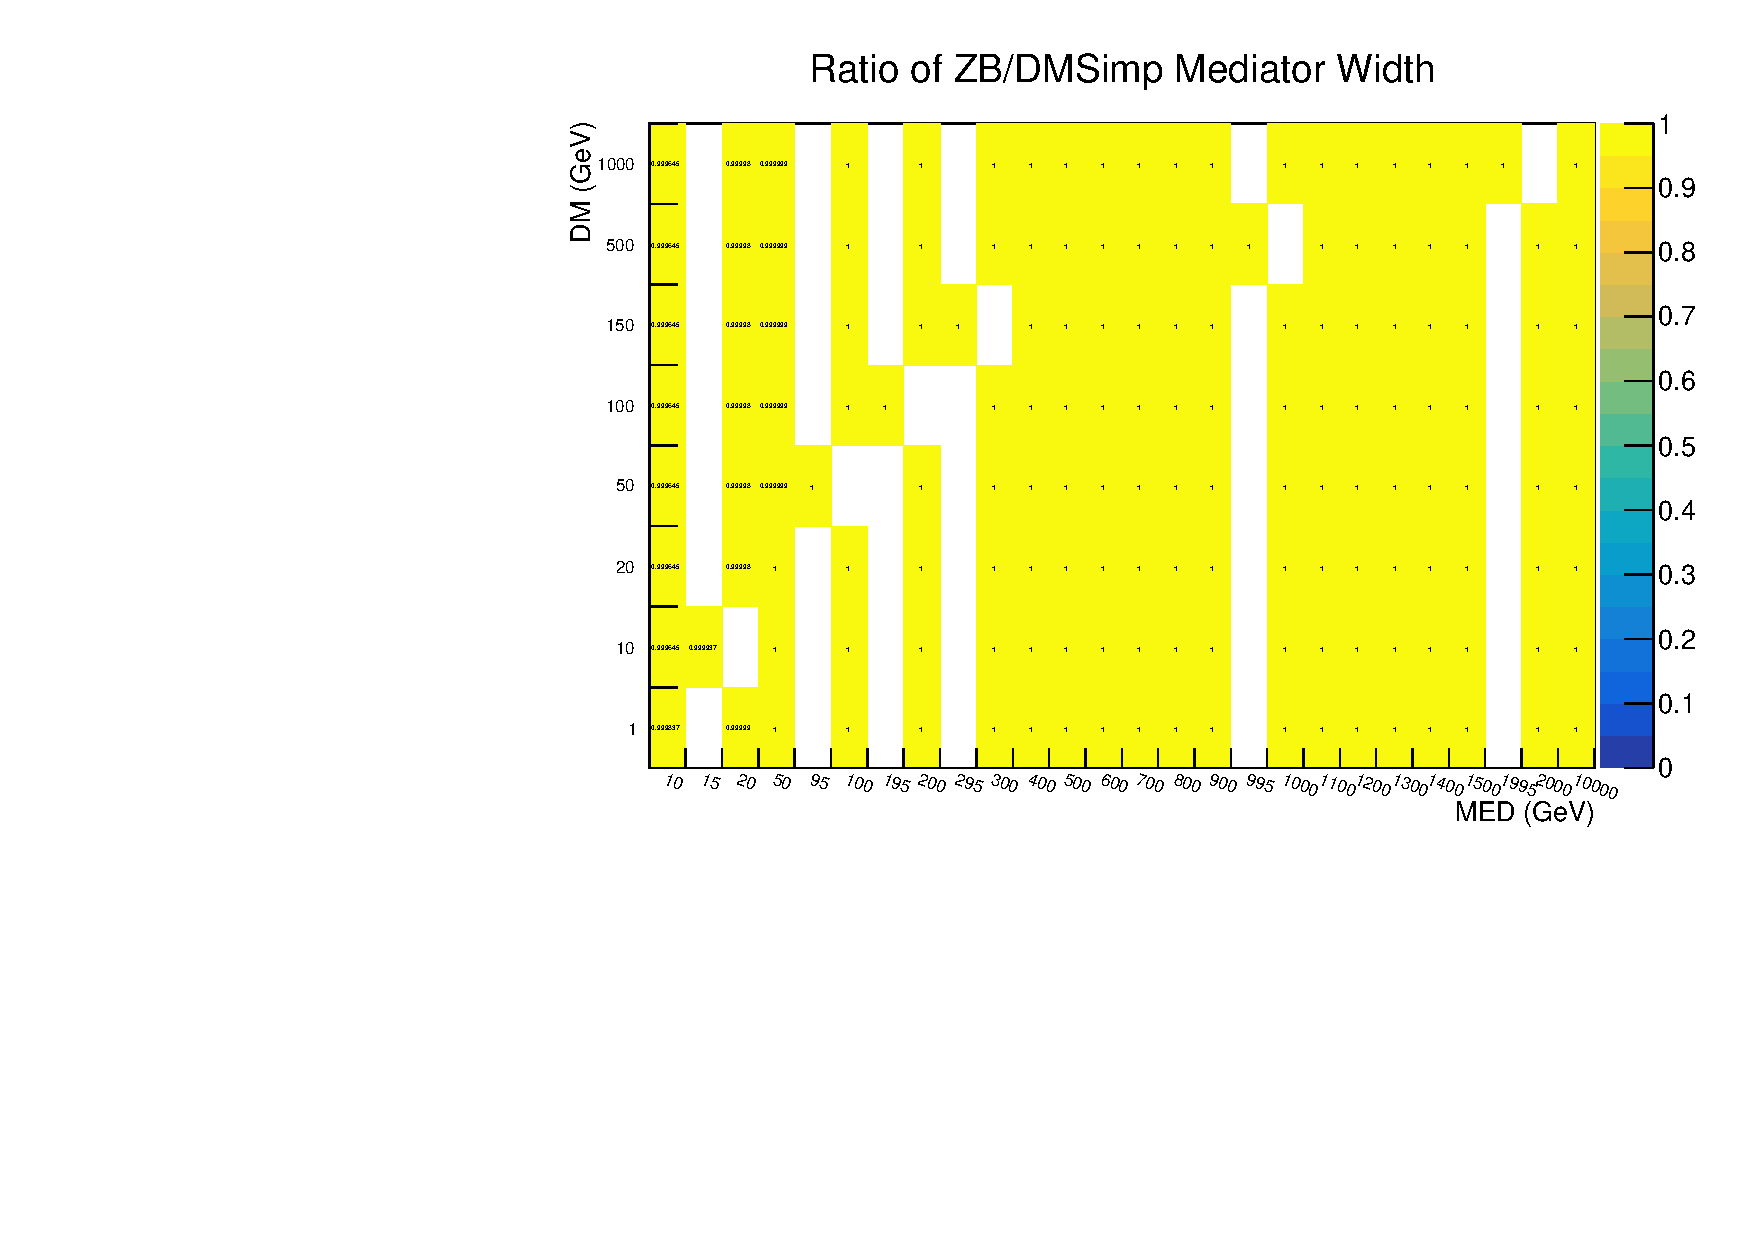
\includegraphics[width=0.45\textwidth]{figures/models/width_ZBToDMSimp.pdf}
%   \caption{Ratios of the leading-order mono-jet cross sections (left) 
%and $\Gamma_{\cPZpr}$ (right) predicted by the \cPZpr-Baryonic model 
%relative to that 
%predicted by {\sc DMSimp-spin1}. The ratios are consistent with unity.
%}
%   \label{fig:ZBXsWidth}
%\end{figure}



%%%%%%%%%%%%%%%%%%%%%%%%%%%%%%%%
%The \MET distributions for many different mass combinations for both models investigated are shown in Fig.~\ref{fig:puppimet_models}. 

%\begin{figure}[htbp]
%   \centering
%   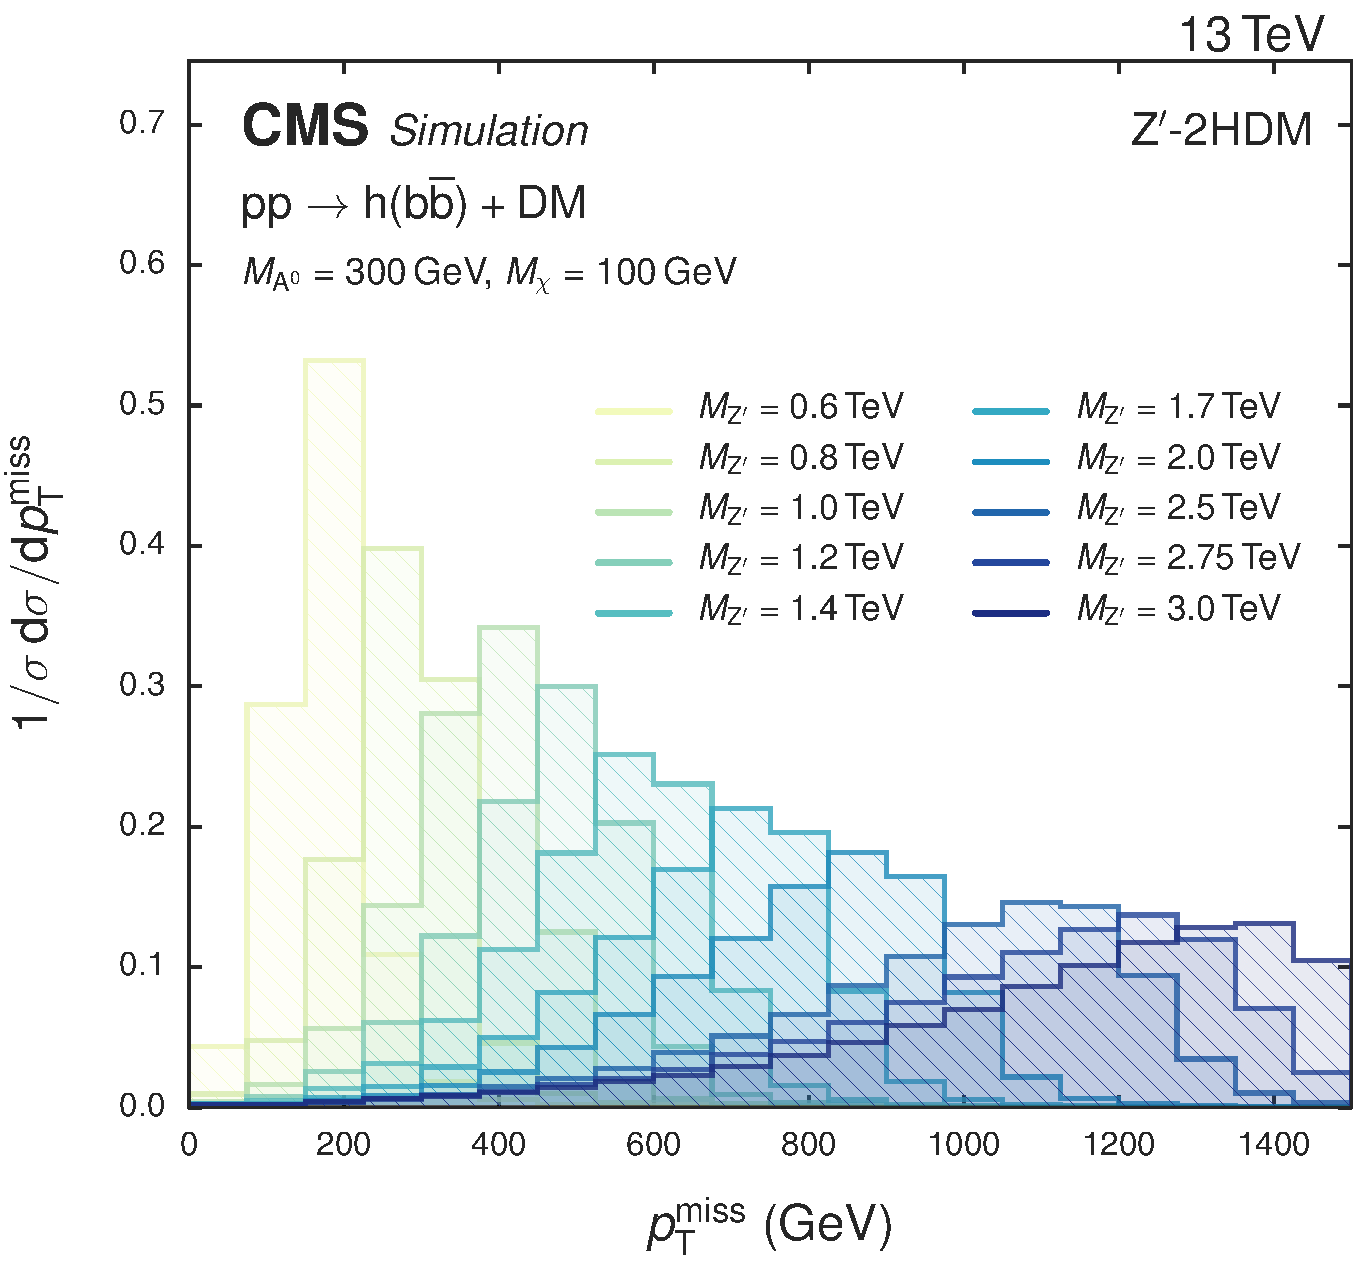
\includegraphics[width=0.43\textwidth]{figures/models/puppimet_signals_2hdm.pdf}
%   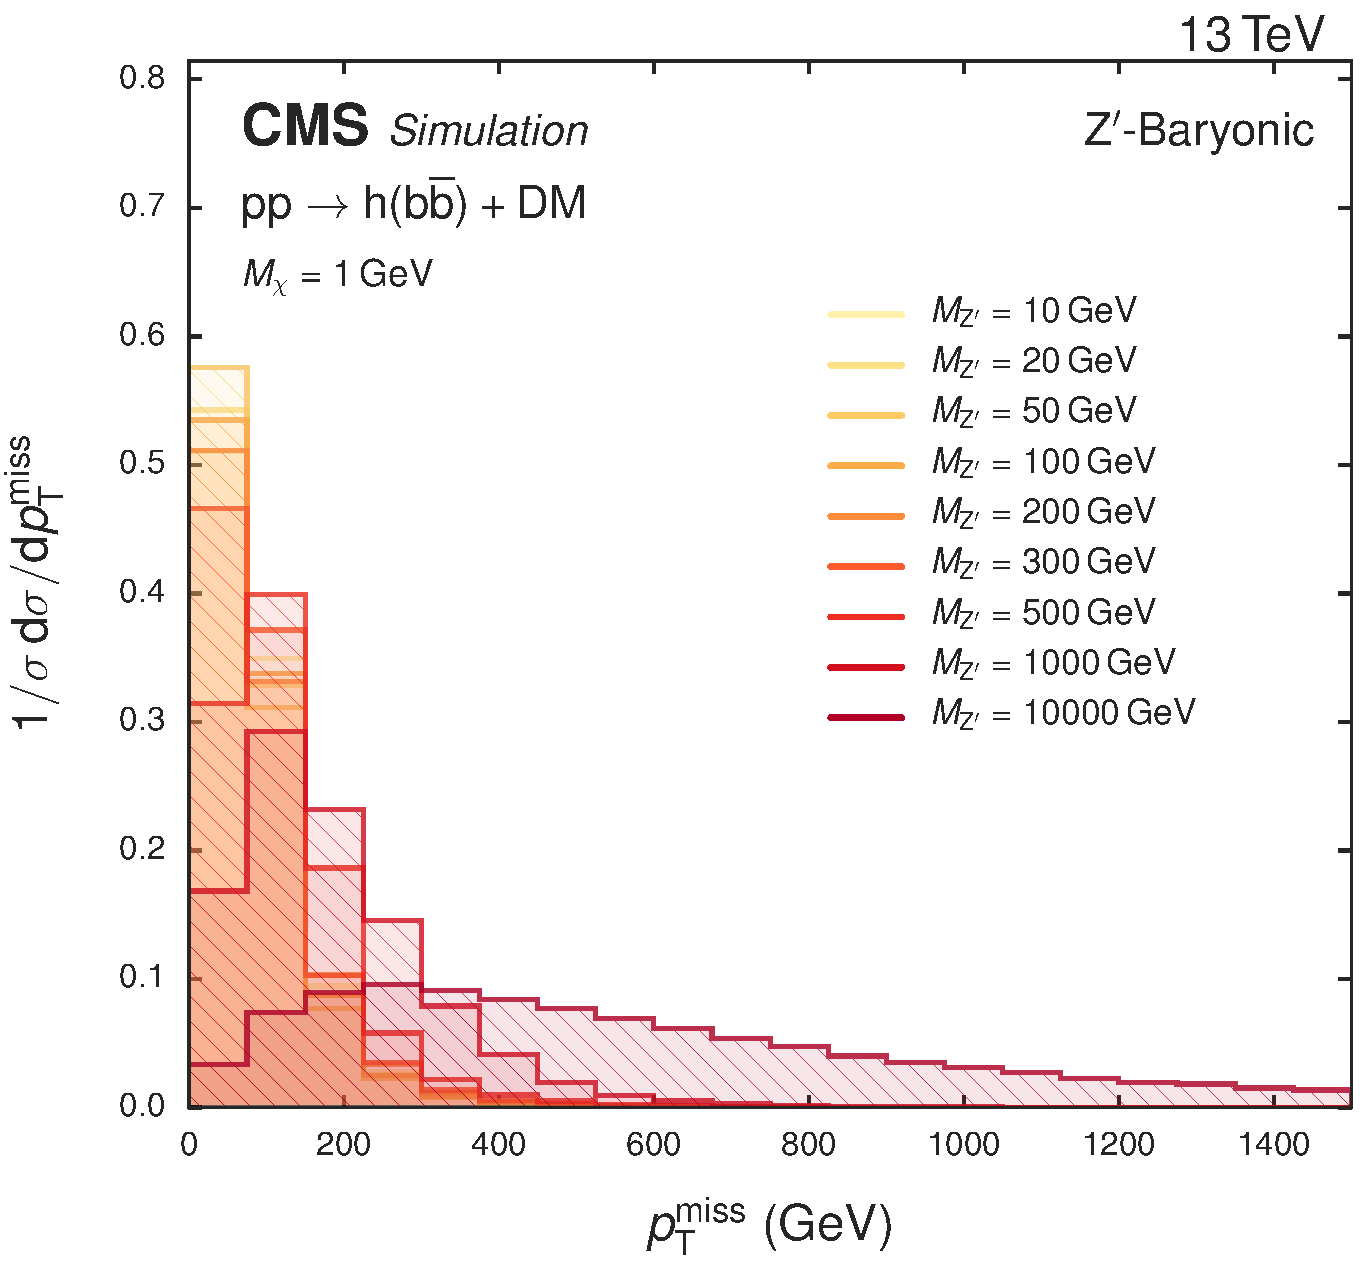
\includegraphics[width=0.43\textwidth]{figures/models/puppimet_signals_barzp.pdf}\\
%   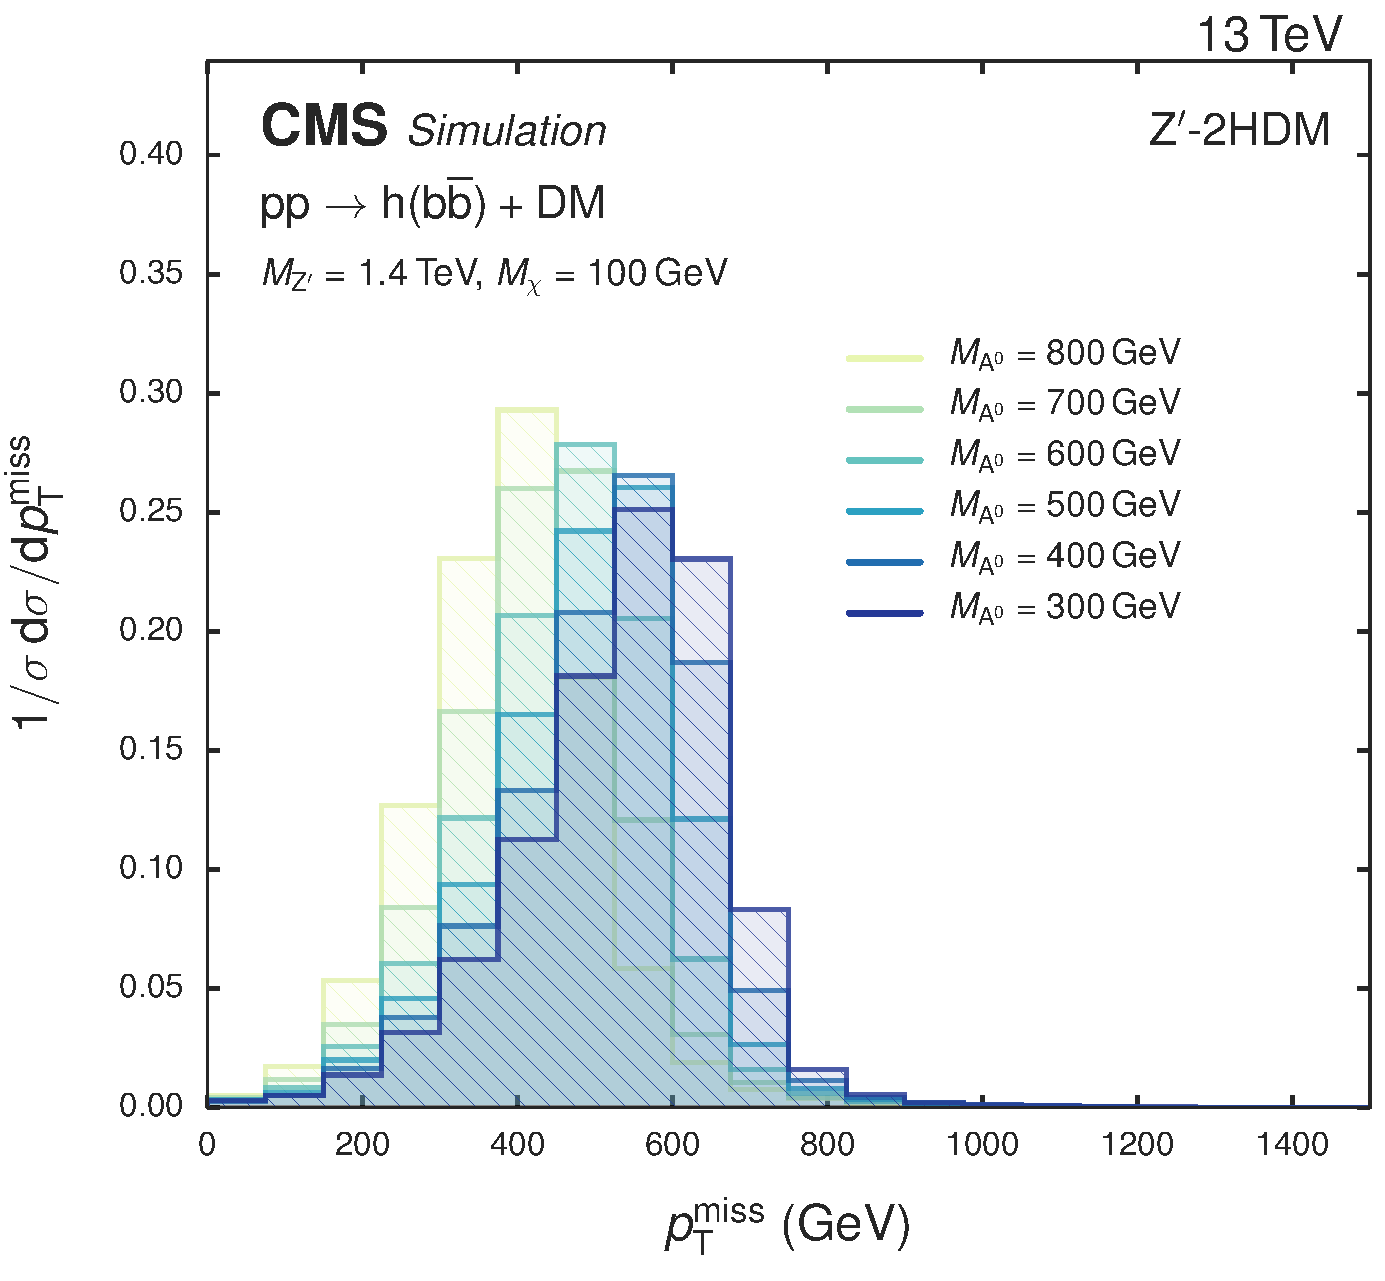
\includegraphics[width=0.43\textwidth]{figures/models/puppimet_signals_2hdm-300.pdf}
%   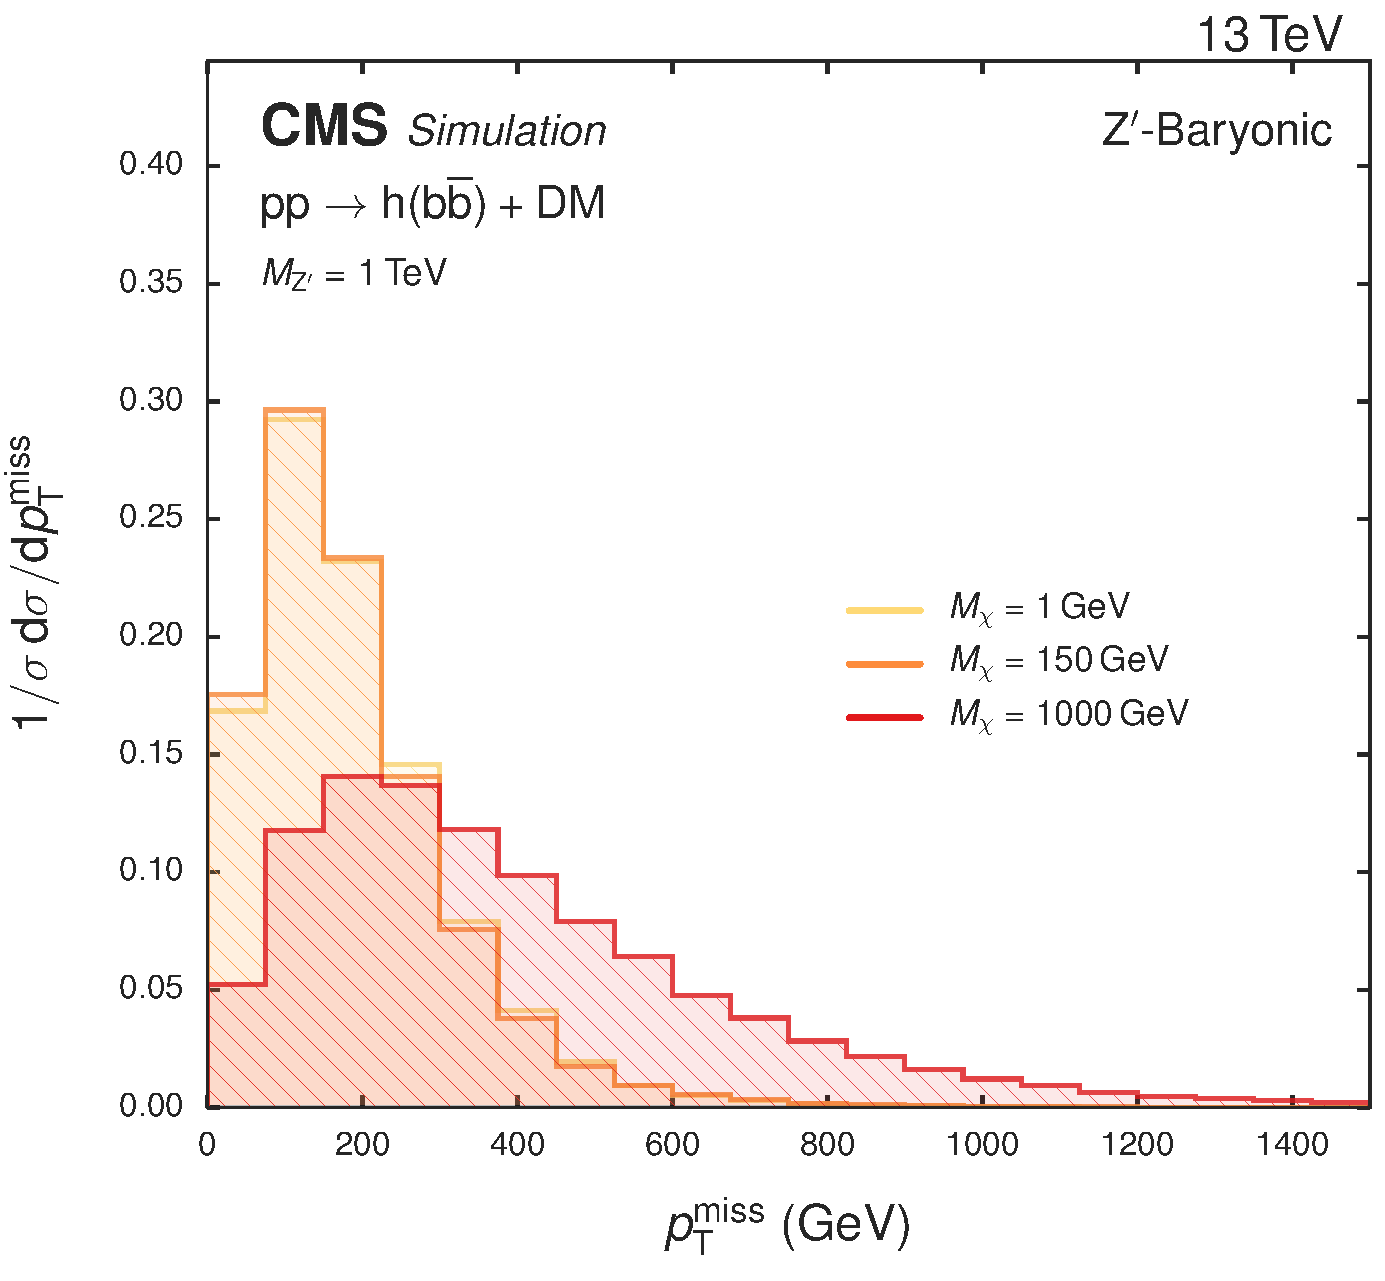
\includegraphics[width=0.43\textwidth]{figures/models/puppimet_signals_barzp-1000.pdf}\\
%   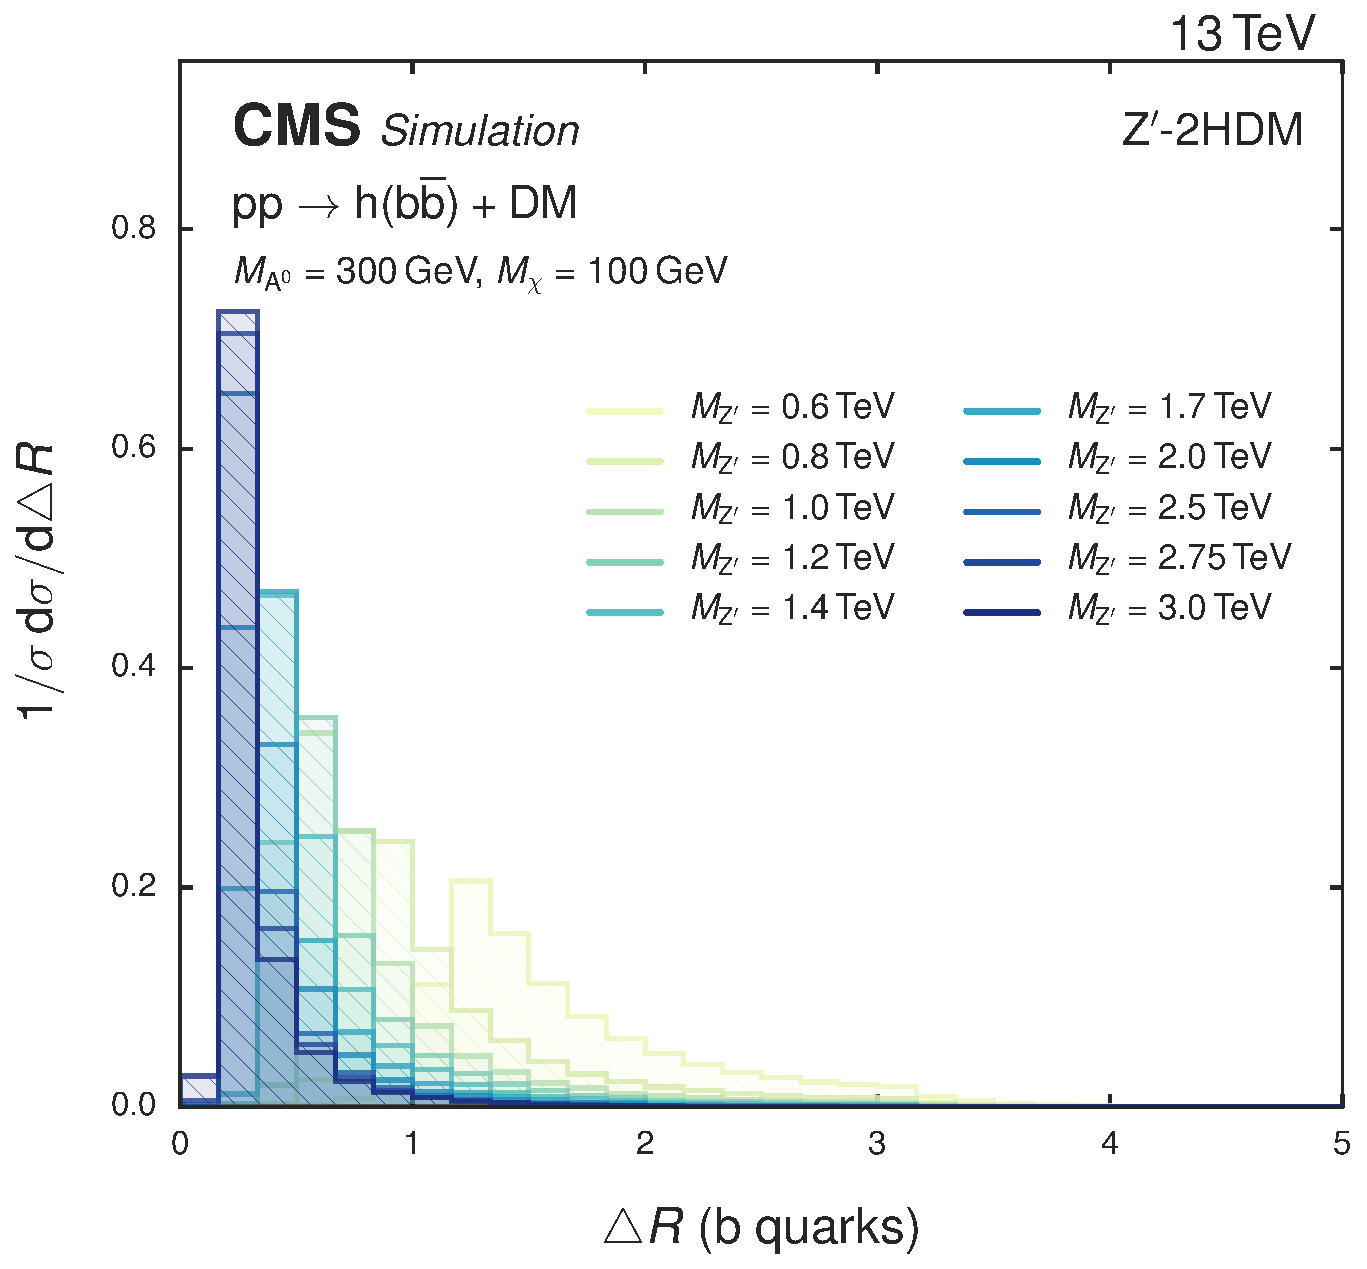
\includegraphics[width=0.43\textwidth]{figures/models/bbdR_signals_2hdm.pdf}
%   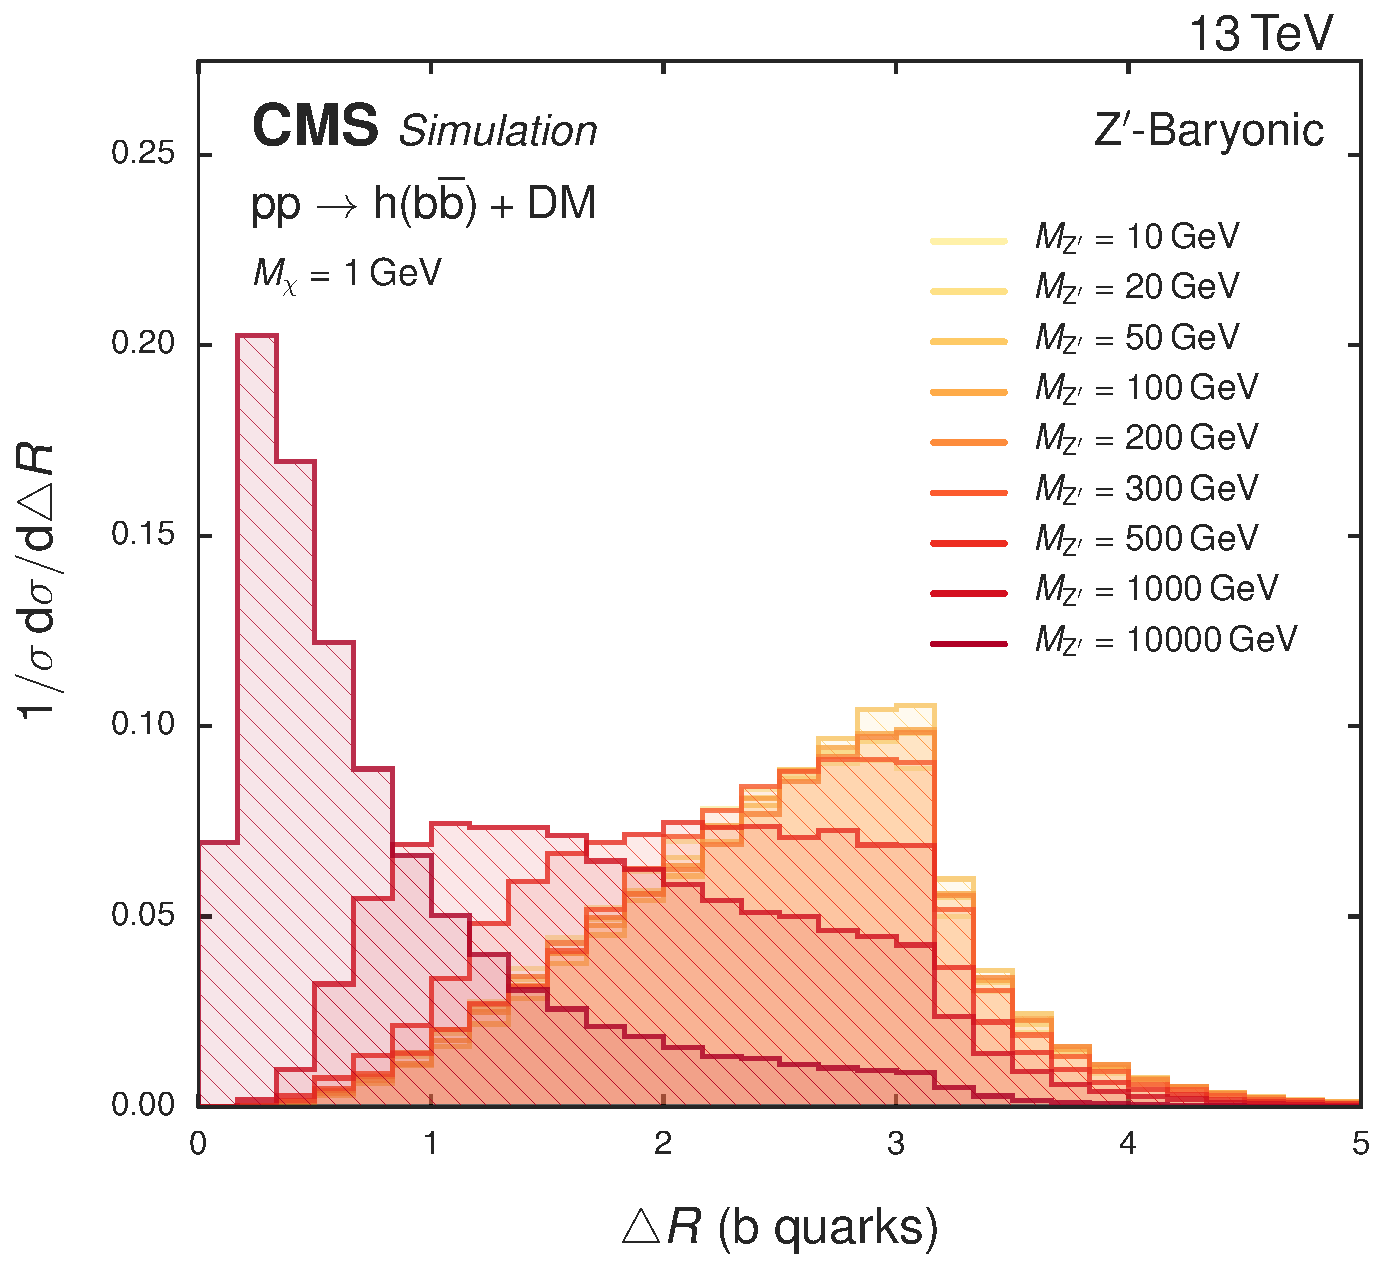
\includegraphics[width=0.43\textwidth]{figures/models/bbdR_signals_barzp.pdf}\\
%   \caption{\ptmiss distributions  for different $M_{\text{Z'}}$ for the Z'-2HDM (upper left) and for the Z'-Baryonic model (upper right); \ptmiss distributions for different $M_{A^0}$ in the Z'-2HDM (middle left) and for different $M_\chi$ (middle right). Lower row: distance between the two b quarks coming from the Higgs boson decay.}
%   \label{fig:puppimet_models}
%\end{figure}


%A direct comparison of the \MET~spectra for the \cPZpr-2HDM and the Baryonic $Z'$ model for similar $M_{\text{Z'}}$ are shown in Fig.~\ref{fig:puppimet_signals}.

%\begin{figure}
%   \centering
%   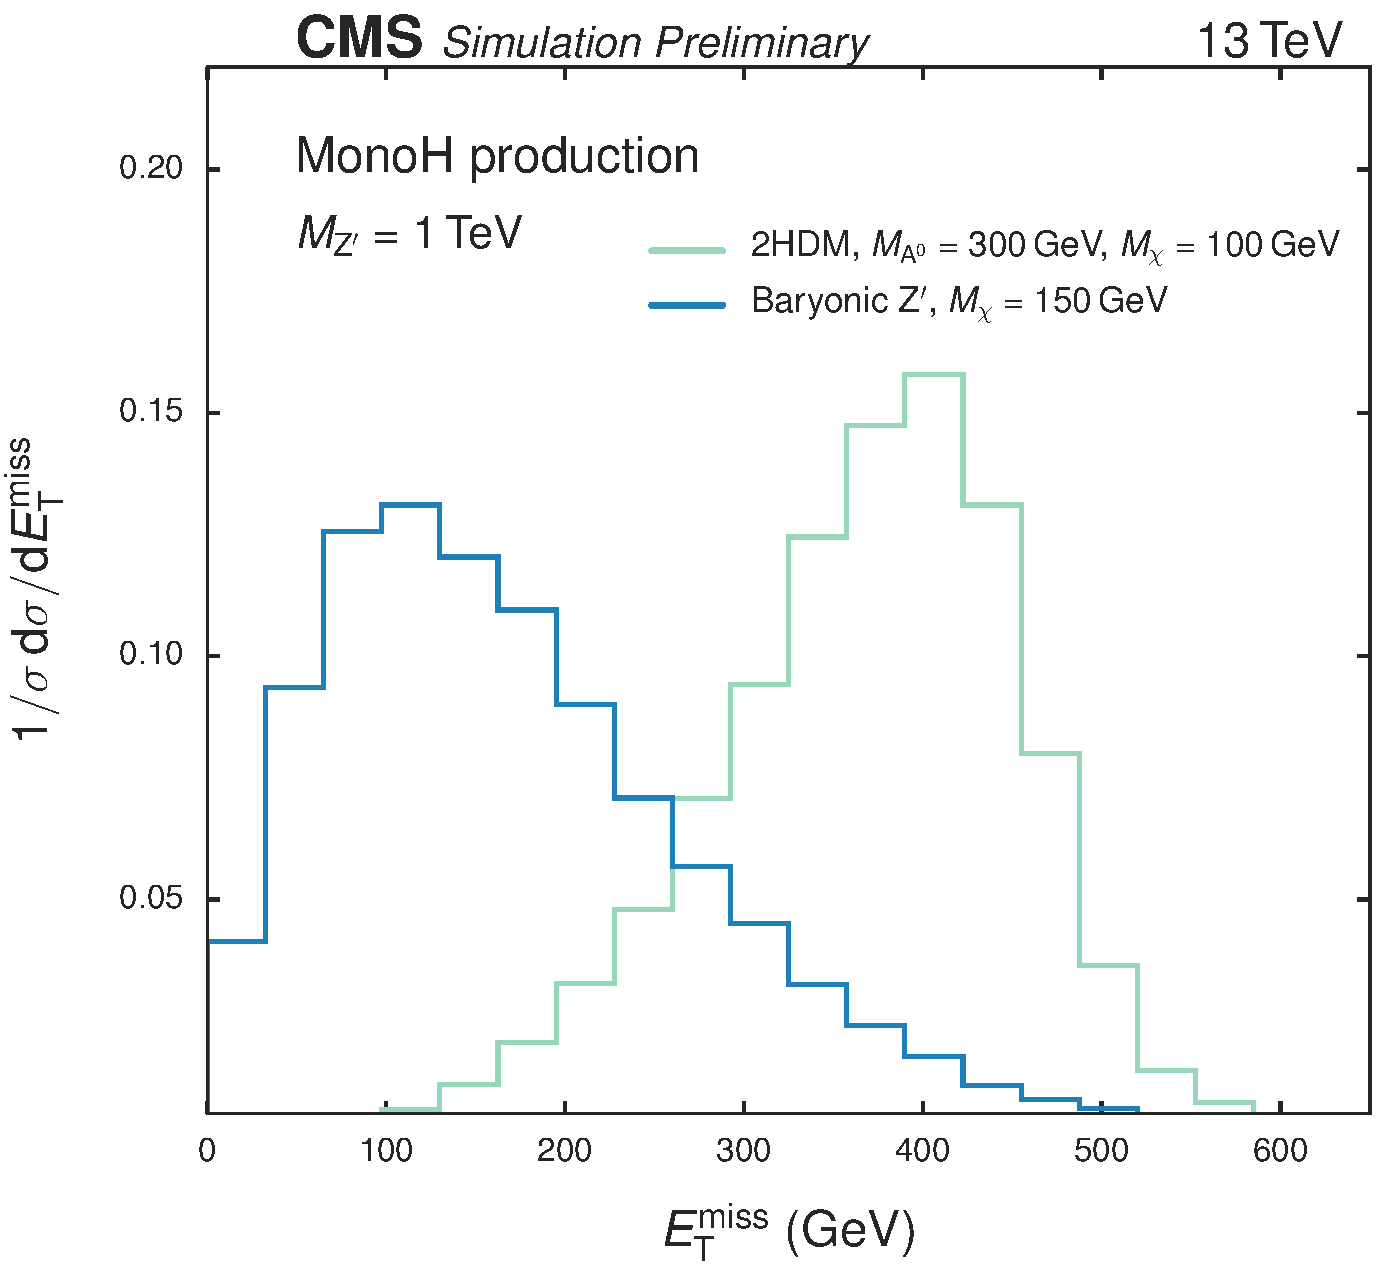
\includegraphics[width=0.6\textwidth]{figures/puppimet_signals.pdf}
%   \caption{\ETslash~spectra for the signal models investigated. The Baryonic $Z'$ model has a significantly softer spectrum.}
%   \label{fig:puppimet_signals}
%\end{figure}
